\documentclass{article}
\usepackage[T1]{fontenc}
\usepackage{lmodern}
\usepackage[polish]{babel}
\usepackage{graphicx}
\usepackage{float}
\usepackage{hyperref}
\usepackage{amsmath}
\usepackage{multicol}
\usepackage{caption}

\usepackage[a4paper, margin=2.54cm]{geometry}

\title{Sprawozdanie - Projekt 3 \\ Aproksymacja profilu wysokościowego \\
Metoda Lagrange'a oraz splajnów}
\author{Damian Jankowski s188597}
\date{25 maja 2023}

\begin{document}

\maketitle

\tableofcontents

\section{Wstęp}

Celem projektu było zaimplementowanie dwóch metod interpolacji: 
metody Lagrange'a i metody wykorzystującej funkcje sklejane trzeciego stopnia
oraz porównanie ich działania na podstawie wybranego profilu wysokościowego.

\section{Opis metod}

\subsection{Metoda interpolacji Lagrange'a}

Metoda Lagrange'a polega na znalezieniu wielomianu $F(x)$, który składa się z funkcji określonych wzorem:
\begin{equation}
   \phi_i(x) = \prod_{j=0, j \neq i}^{n} \frac{x - x_j}{x_i - x_j}, \quad i = 0, 1, \dots, n
\end{equation}
gdzie:
\begin{itemize}
    \item $n$ - liczba węzłów interpolacji
\end{itemize}

Każdy z tych wielomianów spełnia następujący warunek:
\begin{equation}
    \phi_i(x_j) = \begin{cases}
        1 & \text{dla } i = j \\
        0 & \text{dla } i \neq j
    \end{cases}
\end{equation}

Wielomian $F(x)$ można zapisać jako sumę iloczynów wartości funkcji w węźle $x_i$ oraz
postaci wielomianu $\phi_i(x)$ w tym punkcie:
\begin{equation}
    F(x) = \sum_{i=0}^{n} f(x_i) \phi_i(x)
\end{equation}

\subsection{Metoda interpolacji funkcjami sklejanymi (splajnami) trzeciego stopnia}

Metoda interpolacji funkcjami sklejanymi polega na znalezieniu dla każdego
podprzedziału stworzonego z sąsiednich węzłów
interpolacji $[x_i, x_{i+1}]$ wielomianu trzeciego stopnia $S_i(x)$:
\begin{equation}
    S_i(x) = a_i + b_i(x - x_i) + c_i(x - x_i)^2 + d_i(x - x_i)^3
\end{equation}
gdzie:
\begin{itemize}
    \item $a_i, b_i, c_i, d_i$ - szukane współczynniki wielomianu $S_i(x)$
    \item $x_i$ - początek podprzedziału
\end{itemize}

Gdy mamy $n$ węzłów interpolacji, to mamy $n-1$ podprzedziałów, a więc $n-1$ wielomianów $S_i(x)$
do znalezienia. W celu wyznaczenia współczynników tych wielomianów należy spełnić następujące warunki:
\begin{enumerate}
    \item $S_i(x_i) = f(x_i) \quad  i = 0, 1, \dots, n-1$
    \item $S_i(x_{i+1}) = f(x_{i+1}) \quad  i = 0, 1, \dots, n-1$
    \item $S_i'(x_{i+1}) = S_{i+1}'(x_{i+1}) \quad  i = 0, 1, \dots, n-2$
    \item $S_i''(x_{i+1}) = S_{i+1}''(x_{i+1}) \quad  i = 0, 1, \dots, n-2$
    \item $S_0''(x_0) = S_{n-1}''(x_n) = 0$
\end{enumerate}

\begin{itemize}
    \item Warunki 1. i 2. wynikają z tego, że wielomiany $S_i(x)$ muszą osiągać te same wartości co funkcja $f(x)$ 
    w węzłach interpolacji, jest to warunek konieczny, 
    by wielomiany te były wielomianami interpolacyjnymi.
    \item Warunki 3. i 4. wynikają z tego, że wielomiany $S_i(x)$ oraz $S_{i+1}(x)$ muszą być ciągłe 
    w punkcie $x_{i+1}$. Warunki te są konieczne, by wielomiany te były funkcjami sklejanymi.
    \item Warunek 5. tyczy się początku i końca przedziału interpolacji.

\end{itemize}


Do rozwiązania takiego układu równań można zbudować macierze $A$ oraz $b$ i wykorzystując
jedną z metod rozwiązywania układów równań liniowych, np. metodę eliminacji Gaussa, wyznaczyć
współczynniki $a_i, b_i, c_i, d_i$. Z racji, że musimy wyznaczyć $n$ wielomianów $S_i(x)$,
to musimy rozwiązać $4n$ równań liniowych.

\newpage

\section{Dane wejściowe}

Dane wejściowe to trzy trasy rowerowe w formacie GPX,
które zawierają informacje o współrzędnych geograficznych punktów na 
trasie oraz ich wysokościach.
\begin{itemize}
    \item Trasa 1: Gdańsk - Kąty Rybackie - Gdańsk \\
    Dystans: 114.076 km \\
    Różnica wysokości: 56.400 m \\
    Ilość punktów danych: 18090
    \begin{figure}[H]
        \centering
        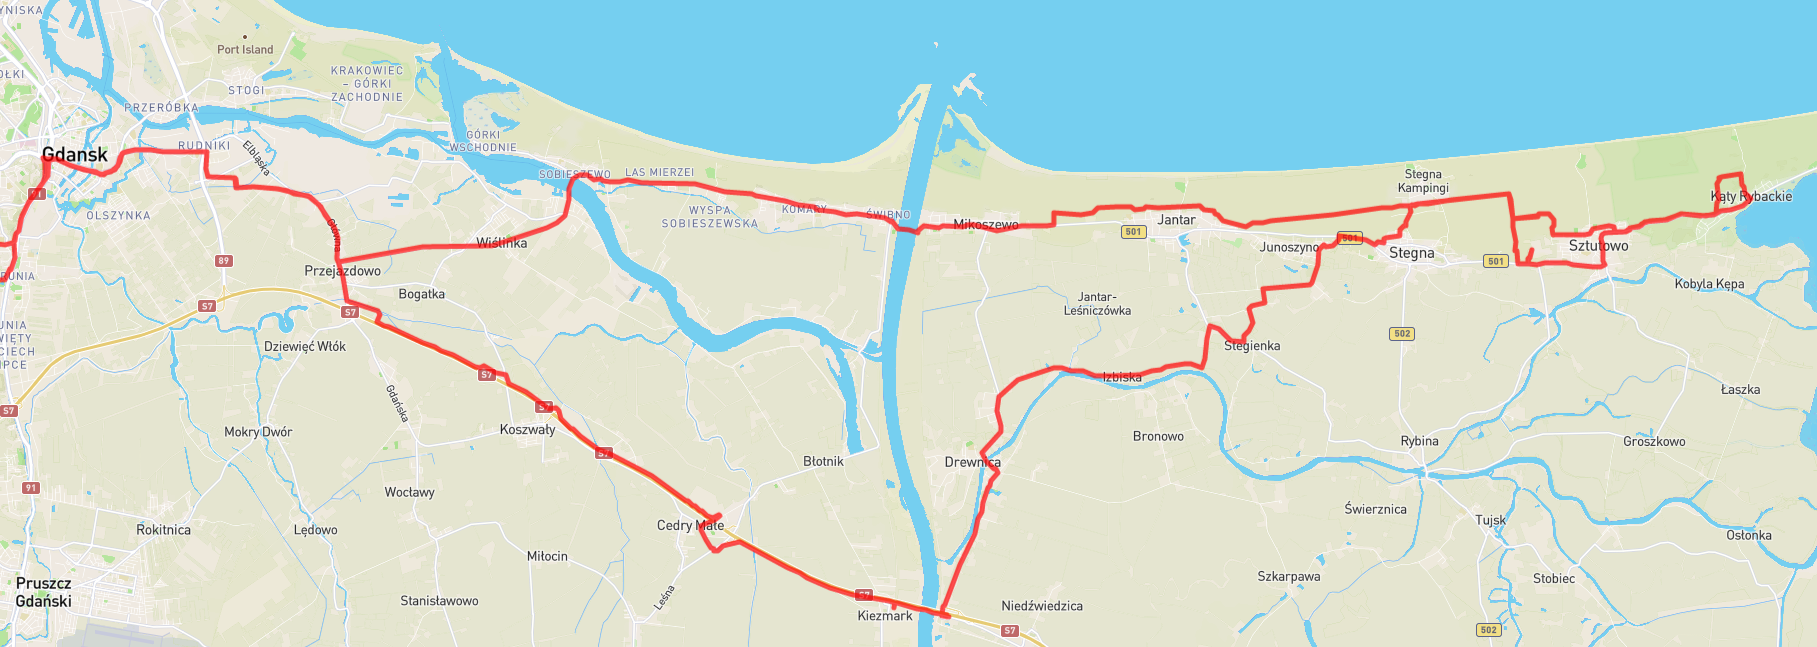
\includegraphics[width=\textwidth]{routes/katy_rybackie.png}
        \caption*{W większości płaska, występują na niej niewielkie 
        różnice wysokości, nie licząc początka i końca trasy}
    \end{figure}
\end{itemize}

\begin{multicols}{2}
    \begin{itemize}
        \item Trasa 2: Gdańsk - Rewa \\
        Dystans: 67.362 km \\
        Różnica wysokości: 168.400 m \\
        Ilość punktów danych: 11889
        \begin{figure}[H]
            \centering
            \captionsetup{justification=centering, width=0.8\linewidth}
            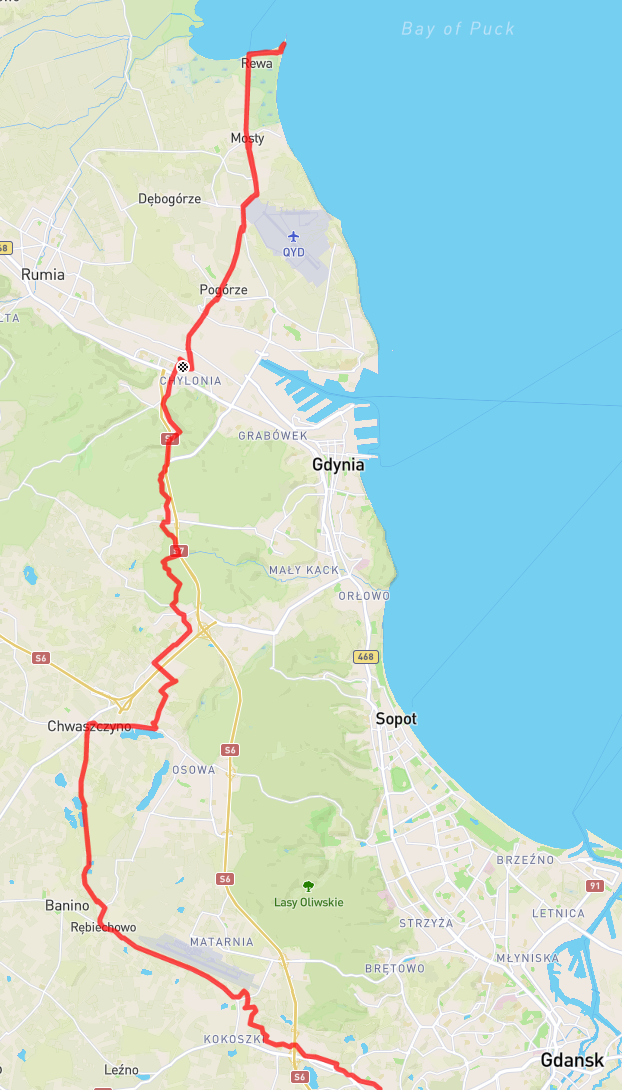
\includegraphics[height=0.35\textheight]{routes/rewa.png}
            \caption*{Odznacza się dużym wzniesieniem oraz kilkoma mniejszymi,
            głównie na końcu trasy}
        \end{figure}

        \item Trasa 3: Gdańsk - Tczew - Gdańsk \\
        Dystans: 80.121 km \\
        Różnica wysokości: 55.300 m \\
        Ilość punktów danych: 14807
        \begin{figure}[H]
            \centering
            \captionsetup{justification=centering, width=0.8\linewidth}
            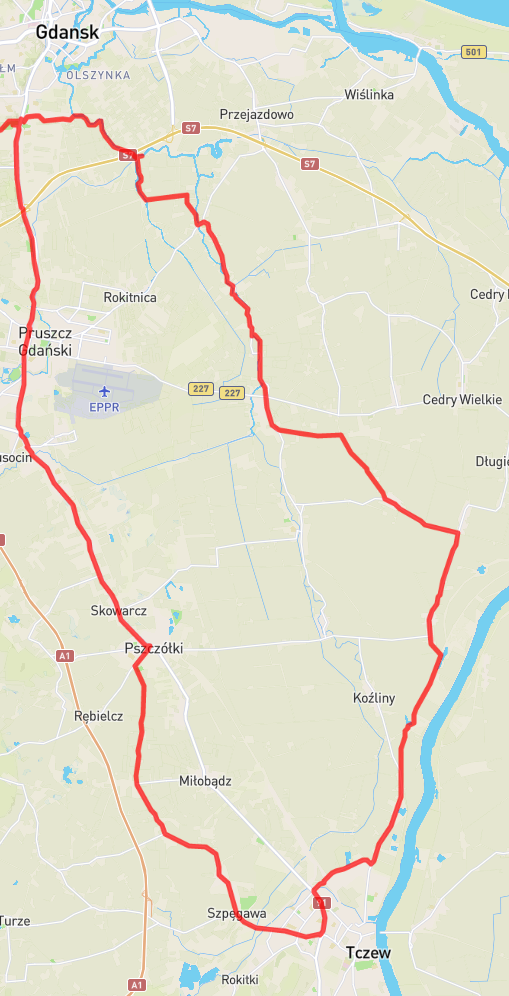
\includegraphics[height=0.35\textheight]{routes/tczew.png}
            \caption*{Zróżnicowana, występują na niej zarówno płaskie odcinki,
            jak również jedno wyraźnie wzniesienie}
        \end{figure}
    \end{itemize}
\end{multicols}

\subsection{Profile wysokościowe}

\begin{figure}[H]
    \centering
    \includegraphics[width=\textwidth]{routes/Gdansk_Katy_Rybackie_profile.png}
    \caption*{Profil wysokościowy \\ \textbf{Trasa 1 - Gdańsk - Kąty Rybackie - Gdańsk}}
\end{figure}

\begin{figure}[H]
    \centering
    \includegraphics[width=\textwidth]{routes/Gdansk_Rewa_profile.png}
    \caption*{Profil wysokościowy \\ \textbf{Trasa 2 - Gdańsk - Rewa}}
\end{figure}

\begin{figure}[H]
    \centering
    \includegraphics[width=\textwidth]{routes/Gdansk_Tczew_profile.png}
    \caption*{Profil wysokościowy \\ \textbf{Trasa 3 - Gdańsk - Tczew - Gdańsk}}
\end{figure}

\newpage

\section{Implementacja}

Wszystkie metody zaimplementowałem w języku \textit{Python} z 
wykorzystaniem biblioteki \textit{numpy} do obliczeń numerycznych
(np. do rozwiązywania układów równań liniowych -- funkcja \textit{numpy.linalg.solve})
oraz biblioteki \textit{matplotlib}
do generowania wykresów.

Każde dwie metody przetestowałem na wcześniej wspomnianych trzech profilach wysokościowych.
Węzły interpolacji wybierałem na dwa sposoby: równomiernie oraz losowo.
Zdecydowałem również o wybraniu różnej ilości węzłów (15 oraz 30), by móc 
zauważyć wpływ ich ilości na dokładność interpolacji.

\begin{itemize}
    \item Plik \texttt{gpx\_parser.py} zawiera funkcje do wczytywania danych z plików GPX,
    a także funkcje pomocnicze do wyznaczania odległości między punktami
    i zwracania listy odległości i wysokości punktów na trasie
    \item Plik \texttt{interpolations.py} zawiera implementacje wcześniej
    wspomnianych metod interpolacji
    \item Plik \texttt{main.py} zawiera funkcje pomocnicze do generowania wykresów
    oraz funkcje do testowania interpolacji
\end{itemize}

\section{Wyniki}

\subsection{Trasa 1}
\subsubsection{Interpolacja Lagrange'a}
\subsubsection*{\hfil 15 węzłów \hfil }

\begin{figure}[H]
    \centering
    \includegraphics[width=\textwidth]{plots/Gdansk_Katy_Rybackie_K=15_Lagrange_unscaled.png}
    \caption{Interpolacja Lagrange'a, 15 węzłów, trasa 1}
\end{figure}

Z racji dużych wahań wartości interpolowanej funkcji, kolejne wykresy będą przeskalowane
do danych rzeczywistych.


\begin{figure}[H]
    \centering
    \includegraphics[width=\textwidth]{plots/Gdansk_Katy_Rybackie_K=15_Lagrange.png}
    \caption{Interpolacja Lagrange'a, 15 węzłów, trasa 1}
\end{figure}

\begin{figure}[H]
    \centering
    \includegraphics[width=\textwidth]{plots/Gdansk_Katy_Rybackie_K=15_Lagrange_random.png}
    \caption{Interpolacja Lagrange'a, 15 węzłów, trasa 1, węzły losowe}
\end{figure}

Z wykresów interpolacji Lagrange'a widać, że metoda ta nie radzi sobie dobrze z interpolacją.
Uwydatnia się tu tzw. efekt Rungego, czyli oscylacje wielomianu interpolacyjnego na krańcach interpolowanego
przedziału. Widać to szczególnie na wykresie z węzłami wybieranymi losowo, gdzie
wielomian interpolacyjny mocno oscyluje w okolicach punktów skrajnych.

\subsubsection*{\hfil 30 węzłów \hfil }
\begin{figure}[H]
    \centering
    \includegraphics[width=\textwidth]{plots/Gdansk_Katy_Rybackie_K=30_Lagrange.png}
    \caption{Interpolacja Lagrange'a, 30 węzłów, trasa 1}
\end{figure}

\begin{figure}[H]
    \centering
    \includegraphics[width=\textwidth]{plots/Gdansk_Katy_Rybackie_K=30_Lagrange_random.png}
    \caption{Interpolacja Lagrange'a, 30 węzłów, trasa 1, węzły losowe}
\end{figure}

Zwiększenie ilości węzłów mocno pogarsza interpolację. Efekt Rungego jest jeszcze bardziej widoczny,
co powoduje, że wielomian interpolacyjny prawie w ogóle nie pokrywa się z danymi wejściowymi.

\subsubsection{Interpolacja splajnami 3. stopnia}

\subsubsection*{\hfil 15 węzłów \hfil }
\begin{figure}[H]
    \centering
    \includegraphics[width=\textwidth]{plots/Gdansk_Katy_Rybackie_K=15_Spline.png}
    \caption{Interpolacja splajnami 3. stopnia, 15 węzłów, trasa 1}
\end{figure}

\begin{figure}[H]
    \centering
    \includegraphics[width=\textwidth]{plots/Gdansk_Katy_Rybackie_K=15_Spline_random.png}
    \caption{Interpolacja splajnami 3. stopnia, 15 węzłów, trasa 1, węzły losowe}
\end{figure}

Interpolacja splajnami 3. stopnia radzi sobie zdecydowanie lepiej niż interpolacja Lagrange'a.
Niewystępowanie efektu Rungego powoduje, że wielomian interpolacyjny dobrze pokrywa się z interpolowanym profilem
wysokościowym. Natomiast losowe wybieranie węzłów podobnie jak w przypadku interpolacji Lagrange'a
przynosi gorsze rezultaty, wszystko zależy od szczęścia w wyborze węzłów. Punkty bliżej siebie
mogą powodować, że wielomian interpolacyjny będzie mocno oscylował w ich okolicach.


\subsubsection*{\hfil 30 węzłów \hfil }
\begin{figure}[H]
    \centering
    \includegraphics[width=\textwidth]{plots/Gdansk_Katy_Rybackie_K=30_Spline.png}
    \caption{Interpolacja splajnami 3. stopnia, 30 węzłów, trasa 1}
\end{figure}


\begin{figure}[H]
    \centering
    \includegraphics[width=\textwidth]{plots/Gdansk_Katy_Rybackie_K=30_Spline_random.png}
    \caption{Interpolacja splajnami 3. stopnia, 30 węzłów, trasa 1, węzły losowe}
\end{figure}

Zwiększenie ilości węzłów znacząco poprawia interpolację. Widać to na wykresie z węzłami równomiernymi,
gdzie wielomian interpolacyjny dość dobrze pokrywa się z danymi wejściowymi. W przypadku węzłów losowych
widać problem z oscylacjami, jednak nie są one tak duże jak w przypadku interpolacji Lagrange'a.


\subsection{Trasa 2}

\subsubsection{Interpolacja Lagrange'a}

\subsubsection*{\hfil 15 węzłów \hfil }

\begin{figure}[H]
    \centering
    \includegraphics[width=\textwidth]{plots/Gdansk_Rewa_K=15_Lagrange.png}
    \caption{Interpolacja Lagrange'a, 15 węzłów, trasa 2}
\end{figure}

\begin{figure}[H]
    \centering
    \includegraphics[width=\textwidth]{plots/Gdansk_Rewa_K=15_Lagrange_random.png}
    \caption{Interpolacja Lagrange'a, 15 węzłów, trasa 2, węzły losowe}
\end{figure}

Podobnie jak w przypadku trasy 1, interpolacja Lagrange'a nie radzi sobie dobrze z interpolacją.
W granicach interpolowanego przedziału wielomian interpolacyjny mocno oscyluje, co powoduje
znaczną rozbieżność z danymi wejściowymi. Profil trasy również nie pomaga, ponieważ jest on
bardziej nieregularny niż w przypadku trasy 1.

\subsubsection*{\hfil 30 węzłów \hfil }

\begin{figure}[H]
    \centering
    \includegraphics[width=\textwidth]{plots/Gdansk_Rewa_K=30_Lagrange.png}
    \caption{Interpolacja Lagrange'a, 30 węzłów, trasa 2}
\end{figure}

\begin{figure}[H]
    \centering
    \includegraphics[width=\textwidth]{plots/Gdansk_Rewa_K=30_Lagrange_random.png}
    \caption{Interpolacja Lagrange'a, 30 węzłów, trasa 2, węzły losowe}
\end{figure}

Bez względu na sposób wyboru węzłów, funkcja interpolowana metodą Lagrange'a nie jest zadowalająca.
Na wykresie z węzłami wybranymi losowo nie da się nawet zauważyć odcinka interpolowanego profilu,
ponieważ wielomian interpolacyjny zwraca bardzo chaotyczne wartości.

\subsubsection{Interpolacja splajnami 3. stopnia}

\subsubsection*{\hfil 15 węzłów \hfil }

\begin{figure}[H]
    \centering
    \includegraphics[width=\textwidth]{plots/Gdansk_Rewa_K=15_Spline.png}
    \caption{Interpolacja splajnami 3. stopnia, 15 węzłów, trasa 2}
\end{figure}

\begin{figure}[H]
    \centering
    \includegraphics[width=\textwidth]{plots/Gdansk_Rewa_K=15_Spline_random.png}
    \caption{Interpolacja splajnami 3. stopnia, 15 węzłów, trasa 2, węzły losowe}
\end{figure}

Interpolacja splajnami 3. stopnia radzi sobie lepiej niż interpolacja Lagrange'a, 
natomiast mała ilość węzłów powoduje, że wielomian interpolacyjny nie pokrywa się
z gwałtownymi zmianami profilu trasy.

\subsubsection*{\hfil 30 węzłów \hfil }

\begin{figure}[H]
    \centering
    \includegraphics[width=\textwidth]{plots/Gdansk_Rewa_K=30_Spline.png}
    \caption{Interpolacja splajnami 3. stopnia, 30 węzłów, trasa 2}
\end{figure}

\begin{figure}[H]
    \centering
    \includegraphics[width=\textwidth]{plots/Gdansk_Rewa_K=30_Spline_random.png}
    \caption{Interpolacja splajnami 3. stopnia, 30 węzłów, trasa 2, węzły losowe}
\end{figure}

Podobnie jak w przypadku pierwszej trasy, zwiększenie ilości węzłów poprawiło aproksymację profilu.
Funkcja interpolowana splajnami 3. stopnia jest gładka, nie ma w niej dużych oscylacji,
a jej wartości są zbliżone do wartości funkcji interpolowanej. Problemem jest jednak
wybór węzłów, ponieważ w przypadku pechowego losowania, funkcja źle przewidzi gwałtowne zmiany profilu.

\subsection{Trasa 3}

\subsubsection{Interpolacja Lagrange'a}

\subsubsection*{\hfil 15 węzłów \hfil }

\begin{figure}[H]
    \centering
    \includegraphics[width=\textwidth]{plots/Gdansk_Tczew_K=15_Lagrange.png}
    \caption{Interpolacja Lagrange'a, 15 węzłów, trasa 3}
\end{figure}

\begin{figure}[H]
    \centering
    \includegraphics[width=\textwidth]{plots/Gdansk_Tczew_K=15_Lagrange_random.png}
    \caption{Interpolacja Lagrange'a, 15 węzłów, trasa 3, węzły losowe}
\end{figure}

Profil trasy 3 jest najbardziej nieregularny ze wszystkich trzech tras. W przypadku interpolacji
Lagrange'a, wielomian interpolacyjny zdecydowanie nie radzi sobie z aproksymacją profilu.

\subsubsection*{\hfil 30 węzłów \hfil }

\begin{figure}[H]
    \centering
    \includegraphics[width=\textwidth]{plots/Gdansk_Tczew_K=30_Lagrange.png}
    \caption{Interpolacja Lagrange'a, 30 węzłów, trasa 3}
\end{figure}

\begin{figure}[H]
    \centering
    \includegraphics[width=\textwidth]{plots/Gdansk_Tczew_K=30_Lagrange_random.png}
    \caption{Interpolacja Lagrange'a, 30 węzłów, trasa 3, węzły losowe}
\end{figure}

Zwiększenie ilości węzłów pogarsza aproksymację profilu trasy 3. W przypadku węzłów równoodległych
widzimy mocny wpływ efektu Rungego, natomiast w przypadku węzłów losowych, wielomian interpolacyjny
przyjmuje bardzo zróżnicowane i nieprzewidywalne wartości.

\subsubsection{Interpolacja splajnami 3. stopnia}

\subsubsection*{\hfil 15 węzłów \hfil }

\begin{figure}[H]
    \centering
    \includegraphics[width=\textwidth]{plots/Gdansk_Tczew_K=15_Spline.png}
    \caption{Interpolacja splajnami 3. stopnia, 15 węzłów, trasa 3}
\end{figure}

\begin{figure}[H]
    \centering
    \includegraphics[width=\textwidth]{plots/Gdansk_Tczew_K=15_Spline_random.png}
    \caption{Interpolacja splajnami 3. stopnia, 15 węzłów, trasa 3, węzły losowe}
\end{figure}

Interpolacja splajnami 3. stopnia po raz kolejny radzi sobie lepiej niż interpolacja Lagrange'a.
Nawet w przypadku wybrania tylko 15 węzłów, wielomian interpolacyjny aproksymuje profil trasy
w sposób zadowalający.

\subsubsection*{\hfil 30 węzłów \hfil }

\begin{figure}[H]
    \centering
    \includegraphics[width=\textwidth]{plots/Gdansk_Tczew_K=30_Spline.png}
    \caption{Interpolacja splajnami 3. stopnia, 30 węzłów, trasa 3}
\end{figure}

\begin{figure}[H]
    \centering
    \includegraphics[width=\textwidth]{plots/Gdansk_Tczew_K=30_Spline_random.png}
    \caption{Interpolacja splajnami 3. stopnia, 30 węzłów, trasa 3, węzły losowe}
\end{figure}

Podwojenie ilości węzłów interpolacji dla tej metody polepszyło aproksymację,
podobnie jak w przypadku dwóch poprzednich profili. 
Natomiast wszystko zależy od tego, w jaki sposób zostały wybrane. 
W przypadku węzłów równoodległych, wielomian interpolacyjny
radzi sobie dobrze, natomiast w przypadku węzłów losowych, funkcja interpolowana
może oscylować w miejscach, gdzie wylosowano blisko siebie wiele węzłów.

\newpage

\section{Wnioski}

\begin{itemize}
    \item Interpolacja Lagrange'a jest wrażliwa na efekt Rungego, 
    który odznacza się dużymi oscylacjami w przypadku interpolacji 
    wielomianowej przy równoodległych węzłach. Dlatego zaleca się wybór 
    mniejszej ilości węzłów w celu zmniejszenia tego efektu.

    \item Interpolacja funkcjami sklejanymi 3. stopnia radzi sobie 
    lepiej z aproksymacją profilu trasy. Dzięki swojej gładkości, funkcja 
    interpolowana nie wykazuje dużych oscylacji i lepiej odzwierciedla 
    rzeczywiste zmiany wysokości terenu.

    \item Zwiększenie ilości węzłów interpolacji często prowadzi do lepszych rezultatów 
    w przypadku interpolacji funkcjami sklejanymi 3. stopnia. Więcej węzłów 
    pozwala na bardziej precyzyjne dopasowanie funkcji interpolującej do danych.

    \item Implementacja interpolacji Lagrange'a jest prostsza i mniej 
    kosztowna pamięciowo oraz obliczeniowo w porównaniu do interpolacji 
    funkcjami sklejanymi 3. stopnia. Lagrange jest oparty na wielomianach 
    interpolacyjnych, podczas gdy splajny wymagają rozwiązania układu równań,
    w którym liczba niewiadomych jest równa pomnożonej przez 4 ilości przedziałów.
    Ta właściwość może być kluczowa, gdy nie zależy nam na dokładności interpolacji,
    a chcemy jak najszybciej otrzymać wynik.

    Z powyższych wniosków wynika, że w przypadku prostych profilów tras, 
    gdzie nie występują duże oscylacje, interpolacja Lagrange'a 
    może być wystarczająca i bardziej efektywna. Jednak w przypadku 
    bardziej złożonych profili terenowych, interpolacja funkcjami 
    sklejanymi 3. stopnia może dawać lepsze rezultaty.
\end{itemize}


\renewcommand{\refname}{Źródła}
\begin{thebibliography}{100}
    \bibitem{intrukcja} 
    Kurs e-nauczanie Metody Numeryczne (Informatyka) - 2023\\
    \textit{Wykład 5}
    \bibitem{wielomianowa}
    Wikipedia, \textit{Interpolacja wielomianowa} \\
    \url{https://pl.wikipedia.org/wiki/Interpolacja_wielomianowa}
    \bibitem{efekt_rungego}
    Wikipedia, \textit{Efekt Rungego} \\
    \url{https://pl.wikipedia.org/wiki/Efekt_Rungego}
    \bibitem{splajny}
    Wikipedia, \textit{Splajn} \\
    \url{https://pl.wikipedia.org/wiki/Splajn}
    \bibitem{interpolacjna_splajnami}
    Wikipedia, \textit{Interpolacja funkcjami sklejanymi} \\
    \url{https://pl.wikipedia.org/wiki/Interpolacja_funkcjami_sklejanymi}

\end{thebibliography}

\end{document}